% -*- latex -*-
%%%%%%%%%%%%%%%%%%%%%%%%%%%%%%%%%%%%%%%%%%%%%%%%%%%%%%%%%%%%%%%%
%%%%%%%%%%%%%%%%%%%%%%%%%%%%%%%%%%%%%%%%%%%%%%%%%%%%%%%%%%%%%%%%
%%%%
%%%% This text file is part of the source of 
%%%% `Parallel Programming in MPI and OpenMP'
%%%% by Victor Eijkhout, copyright 2012-2020
%%%%
%%%% mpi.tex : leftover MPI topics
%%%%
%%%%%%%%%%%%%%%%%%%%%%%%%%%%%%%%%%%%%%%%%%%%%%%%%%%%%%%%%%%%%%%%
%%%%%%%%%%%%%%%%%%%%%%%%%%%%%%%%%%%%%%%%%%%%%%%%%%%%%%%%%%%%%%%%

\lstset{style=reviewcode,language=C}
\Level 0 {Contextual information, attributes, etc.}
\label{sec:context}

\Level 1 {Info objects}
\label{sec:mpi-info}

Certain MPI routines can accept \indexmpiref{MPI_Info} objects.
These contain key-value pairs that can offer system or implementation
dependent information.

Create an info object with \indexmpiref{MPI_Info_create}
and delete it with \indexmpiref{MPI_Info_free}.

Keys are then set with \indexmpiref{MPI_Info_set},
and they can be queried with \indexmpiref{MPI_Info_get}.
Note that the output of the `get' routine is not allocated:
it is a buffer that is passed. 
The maximum length of a key is given by the parameter
\indexmpidef{MPI_MAX_INFO_KEY}.
You can delete a key from an info object with \indexmpiref{MPI_Info_delete}.

There is a straightforward duplication of info objects:
\indexmpiref{MPI_Info_dup}.

You can also query the number of keys in an info object with
\indexmpiref{MPI_Info_get_nkeys},
after which the keys can be queried in succession with
\indexmpidef{MPI_Info_get_nthkey}

Info objects that are marked as `In' or `Inout' arguments
are parsed before that routine returns.
This means that in non-blocking routines they can be freed immediately,
unlike, for instance, send buffers.

\Level 2 {Environment information}
\label{sec:mpi-info-env}

The object \indexmpidef{MPI_INFO_ENV} is predefined, containing:
\begin{itemize}
\item \n{command}
  Name of program executed.
\item  \n{argv}
  Space separated arguments to command.
\item  \n{maxprocs}
  Maximum number of MPI processes to start.
\item   \n{soft}
  Allowed values for number of processors.
\item   \n{host}
  Hostname.
\item   \n{arch}
  Architecture name.
\item   \n{wdir}
  Working directory of the MPI process.
\item   \n{file}
  Value is the name of a file in which additional information is specified.
\item   \n{thread_level}
  Requested level of thread support, if requested before the program started execution.
\end{itemize}
Note that these are the requested values; the running program can for instance
have lower thread support.

\Level 2 {Communicator and window information}

MPI has a built-in possibility of attaching information to
\emph{communicators}\index{communicator!info object}
and
\emph{windows}\index{window!info object}
using the calls
\indexmpishow{MPI_Comm_get_info}
\indexmpishow{MPI_Comm_set_info},
\indexmpishow{MPI_Win_get_info},
\indexmpishow{MPI_Win_set_info}.

Copying a communicator with \indexmpishow{MPI_Comm_dup} would cause
the info to be copied; to attach new information to the copy there is
\indexmpidef{MPI_Comm_dup_with_info}.

\Level 2 {File information}
\label{sec:mpi-file-info}

An \indexmpishow{MPI_Info} object can be passed to the following file routines:
\begin{itemize}
\item \indexmpishow{MPI_File_open}
\item \indexmpishow{MPI_File_set_view}
\item \indexmpishow{MPI_File_set_info}; collective.
\end{itemize}

The following keys are defined in the \mpistandard{2} standard:
\begin{itemize}
\item \indexmpishow{access_style}: A comma separated list of one or
  more of: \n{read_once}, \n{write_once}, \n{read_mostly},
  \n{write_mostly}, \n{sequential}, \n{reverse_sequential}, \n{random}
\item \indexmpishow{collective_buffering}: true or false; enables or disables buffering on collective I/O operations
\item \indexmpishow{cb_block_size}: integer block size for collective buffering, in bytes
\item \indexmpishow{cb_buffer_size}: integer buffer size for collective buffering, in bytes
\item \indexmpishow{cb_nodes}: integer number of MPI processes used in collective buffering
\item \indexmpishow{chunked}: a comma separated list of integers describing the dimensions of a multidimensional array to be accessed using subarrays, starting with the most significant dimension (1st in C, last in Fortran)
\item \indexmpishow{chunked_item}: a comma separated list specifying the size of each array entry, in bytes
\item \indexmpishow{chunked_size}: a comma separated list specifying the size of the subarrays used in chunking
\item \indexmpishow{file_perm}: UNIX file permissions at time of creation, in octal
\item \indexmpishow{io_node_list}: a comma separated list of I/O nodes to use
\item \indexmpishow{nb_proc}: integer number of processes expected to access a file simultaneously
\item \indexmpishow{num_io_nodes}: integer number of I/O nodes to use
\item \indexmpishow{striping_factor}: integer number of I/O nodes/devices a file should be striped across
\item \indexmpishow{striping_unit}: integer stripe size, in bytes
\end{itemize}
Additionally, file system-specific keys can exist.

\Level 1 {Attributes}
\label{sec:mpi_attr}

Some runtime (or installation dependendent) values are available as
attributes through
\indexmpiref{MPI_Comm_get_attr}.
(The MPI-2 routine \indexmpidef{MPI_Attr_get} is deprecated).
The flag parameter has two functions:
\begin{itemize}
\item it returns whether the attributed was found;
\item if on entry it was set to false, the value parameter is ignored
  and the routines only tests whether the key is present.
\end{itemize}
The return value parameter is subtle: while it is declared \lstinline{void*},
it is actually the address of a \lstinline{void*} pointer.

\cverbatimsnippet[examples/mpi/c/tags.c]{gettagub}
\pverbatimsnippet[examples/mpi/p/tags.py]{gettagubp}

Attributes are:
\begin{itemize}
\item \indexmpidef{MPI_TAG_UB}
  Upper bound for \emph{tag value}\index{tag!bound on value}.
  (The lower bound is zero.)
  Note that \indexmpishow{MPI_TAG_UB} is the key, not the actual upper bound!
  This value has to be at least 32767.
\item \indexmpishow{MPI_HOST}
  Host process rank, if such exists, \indexmpishow{MPI_PROC_NULL}, otherwise.
\item \indexmpishow{MPI_IO}
rank of a node that has regular I/O facilities (possibly
myrank). Nodes in the same communicator may return different values
for this parameter.
\item \indexmpishow{MPI_WTIME_IS_GLOBAL}
Boolean variable that indicates whether clocks are synchronized.
\end{itemize}

Also:
\begin{itemize}
\item \indexmpishow{MPI_UNIVERSE_SIZE}: the total number of processes
  that can be created. This can be more than the size of
  \indexmpishow{MPI_COMM_WORLD} if the host list is larger than the number of
  initially started processes. See section~\ref{sec:mpi-dynamic}.

  Python: \lstinline{mpi4py.MPI.UNIVERSE_SIZE}.
\item \indexmpidef{MPI_APPNUM}: if MPI is used in \ac{MPMD} mode, or
  if \indexmpishow{MPI_Comm_spawn_multiple} is used, this attribute
  reports the how-manieth program we are in.
\end{itemize}

\Level 1 {Processor name}

You can query the \indexterm{hostname} of a processor with
\indexmpishow{MPI_Get_processor_name}.
This name need not be unique between different processor ranks.

You have to pass in the character storage:
the character array must be at least \indexmpidef{MPI_MAX_PROCESSOR_NAME} characters long.
The actual length of the name is returned in the \n{resultlen} parameter.

\Level 1 {Version information}

For runtime determination,
The \indextermbus{MPI}{version} is available through two parameters
\indexmpishow{MPI_VERSION} and \indexmpishow{MPI_SUBVERSION}
or the function \indexmpiref{MPI_Get_version}.

\Level 0 {Error handling}
\label{sec:mpi:error}

Errors in normal programs can be tricky to deal with; errors in
parallel programs can be even harder. This is because in addition to
everything that can go wrong with a single executable (floating point
errors, memory violation) you now get errors that come from faulty
interaction between multiple executables.

A few examples of what can go wrong:
\begin{itemize}
\item MPI errors: an MPI routine can abort for various reasons, such
  as receiving much more data than its buffer can accomodate. Such
  errors, as well as the more common type mentioned above, typically
  cause your whole execution to abort. That is, if one incarnation of
  your executable aborts, the MPI runtime will kill all others.
\item Deadlocks and other hanging executions: there are various
  scenarios where your processes individually do not abort, but are all
  waiting for each other. This can happen if two processes are both
  waiting for a message from each other, and this can be helped by
  using non-blocking calls. In another scenario, through an error in
  program logic, one process will be waiting for more messages
  (including non-blocking ones) than are sent to it.
\end{itemize}

\Level 1 {Error codes}
\label{sec:mpi-err-codes}

\begin{itemize}
\item \indexmpidef{MPI_ERR_ARG}: an argument was invalid that is not
  covered by another error code.
\item \indexmpidef{MPI_ERR_BUFFER} The buffer pointer is invalid;
  this typically means that you have supplied a null pointer.
\item \indexmpidef{MPI_ERR_COMM}: 
  invalid communicator. A common error is to use a null communicator in
  a call.
\item \indexmpidef{MPI_ERR_INTERN} An internal error in MPI has been detected.
\item \indexmpidef{MPI_ERR_IN_STATUS} A functioning returning an array of statuses
  has at least one status where the \indexmpishow{MPI_ERROR} field is set
  to other than \indexmpishow{MPI_SUCCESS}. See section~\ref{sec:mpi-status-error}.
\item \indexmpidef{MPI_ERR_INFO}: 
  invalid info object.
\item \indexmpidef{MPI_ERR_OTHER}: an error occurred; use
  \indexmpidef{MPI_Error_string} to retrieve further information
  about this error.
\item \indexmpidef{MPI_ERR_PORT}: invalid port; this applies to
  \indexmpishow{MPI_Comm_connect} and such.
\item \indexmpidef{MPI_ERR_SERVICE}: invalid service in
  \indexmpishow{MPI_Unpublish_name}.
\item \indexmpidef{MPI_SUCCESS}: 
  no error; MPI routine completed successfully.
\end{itemize}

\Level 1 {Error handling}
\label{sec:mpi-error}

The MPI library has a general mechanism for dealing with errors that
it detects: one can specify an error handler
with \indexmpishow{MPI_Comm_set_errhandler},
where some handlers of type \indexmpidef{MPI_Errhandler} are predefined.

\begin{remark}
  The routine
  \lstinline{MPI_Errhandler_set} is deprecated.
\end{remark}

\Level 2 {Abort}

The default behaviour, where the full run is aborted, is
equivalent to your code having the following
call to 
\begin{lstlisting}
MPI_Comm_set_errhandler(MPI_COMM_WORLD,MPI_ERRORS_ARE_FATAL);
\end{lstlisting}

The handler \indexmpidef{MPI_ERRORS_ARE_FATAL}, even though it is
associated with a communicator, causes the whole application to abort.

\begin{mpifour}
  % https://github.com/mpi-forum/mpi-issues/issues/3
  The handler \indexmpidef{MPI_ERRORS_ABORT} (\mpistandard{4})
  aborts on the processes in the communicator for which it is specified.
\end{mpifour}

\Level 2 {Return}

Another simple possibility is to specify
\begin{lstlisting}
MPI_Comm_set_errhandler(MPI_COMM_WORLD,MPI_ERRORS_RETURN);
\end{lstlisting}
which causes the error code to be returned to the user.
This gives you the opportunity to write code that handles the error
return value. 

\Level 2 {Error printing}

If the \indexmpishow{MPI_Errhandler} value \indexmpishow{MPI_ERRORS_RETURN} is used,
you can compare the return code to \indexmpidef{MPI_SUCCESS}
and  print out debugging information:

\begin{lstlisting}
int ierr;
ierr = MPI_Something();
if (ierr!=MPI_SUCCESS) {
    // print out information about what your programming is doing
    MPI_Abort();
}
\end{lstlisting}
For instance,
\begin{verbatim}
Fatal error in MPI_Waitall: 
See the MPI_ERROR field in MPI_Status for the error code
\end{verbatim}
You could then retrieve the \indexmpishow{MPI_ERROR} field of the
status, and print out an error string with
\indexmpidef{MPI_Error_string}
or maximal size \indexmpidef{MPI_MAX_ERROR_STRING}:
\begin{lstlisting}
MPI_Comm_set_errhandler(MPI_COMM_WORLD,MPI_ERRORS_RETURN);
ierr = MPI_Waitall(2*ntids-2,requests,status);
if (ierr!=0) {
   char errtxt[MPI_MAX_ERROR_STRING];
   for (int i=0; i<2*ntids-2; i++) {
     int err = status[i].MPI_ERROR;
     int len=MPI_MAX_ERROR_STRING;
     MPI_Error_string(err,errtxt,&len);
     printf("Waitall error: %d %s\n",err,errtxt);
   }
   MPI_Abort(MPI_COMM_WORLD,0);
}
\end{lstlisting}
One cases where errors can be handled is that of \emph{MPI file
  I/O}\index{MPI!I/O}: if an output file has the wrong
permissions, code can possibly progress without writing data, or
writing to a temporary file.

MPI operators (\indexmpishow{MPI_Op}) do not return an error code. In case of
an error they call \indexmpishow{MPI_Abort}; if \indexmpishow{MPI_ERRORS_RETURN}
is the error handler, error codes may be silently ignored.

You can create your own error handler with
\indexmpiref{MPI_Comm_create_errhandler}, which is then installed with
\indexmpishow{MPI_Comm_set_errhandler}. You can retrieve the error
handler with \indexmpishow{MPI_Comm_get_errhandler}.

\begin{mplnote}{Communicator errhandler}
  \ac{MPL} does not allow for access to the wrapped communicators.
  However, for \indexmpishow{MPI_COMM_WORLD}, the routine
  \indexmpishow{MPI_Comm_set_errhandler}
  can be called directly.
\end{mplnote}

\Level 0 {Fortran issues}
\label{sec:mpi-fortran}
\index{MPI!Fortran issues|see{Fortran, MPI issues}}
\index{Fortran!MPI issues|(}

MPI is typically written in C, what if you program \emph{Fortran}?

See section~\ref{sec:f90-types} for MPI types corresponding to
\emph{Fortran90 types}\index{Fortran90 types!in MPI}.

\Level 1 {Assumed-shape arrays}\index{Fortran!assumed-shape arrays in MPI}
\label{sec:mpif-shape}

Use of other than contiguous data, for instance \n{A(1:N:2)}, was a
problem in MPI calls, especially non-blocking ones. In that case it
was best to copy the data to a contiguous array. This has been fixed
in \indextermbus{MPI}{3}.

\begin{itemize}
\item Fortran routines have the same prototype as C~routines except for the addition
  of an integer error parameter.
\item The call for
  %\indexmpishowsub{MPI_Init}{in Fortran}
  \indexmpishowf{MPI_Init} in Fortran
  does not have the commandline arguments;
  they need to be handled separately.
\item The routine \indexmpishow{MPI_Sizeof} is only available in
  Fortran, it provides the functionality of the C/C++ operator
  \indextermtt{sizeof}.
\end{itemize}

\index{Fortran!MPI issues|)}

\Level 0 {Fault tolerance}
\label{mpi:tolerant}

Processors are not completely reliable, so it may happen that one
`breaks': for software or hardware reasons it becomes
unresponsive. For an MPI program this means that it becomes impossible
to send data to it, and any collective operation involving it will
hang. Can we deal with this case? Yes, but it involves some
programming.

First of all, one of the possible MPI error return codes
(section~\ref{sec:mpi:error}) is \indexmpishow{MPI_ERR_COMM}, which can be returned
if a processor in the communicator is unavailable. You may want to
catch this error, and add a `replacement processor' to the
program. For this, the \indexmpishow{MPI_Comm_spawn} can be used
(see~\ref{sec:mpi-dynamic} for details).
%
But this requires a change of program design: the communicator
containing the new process(es) is not part of the
old \indexmpishow{MPI_COMM_WORLD}, so it is better to set up your code as a
collection of inter-communicators to begin with.

\Level 0 {Local and non-local operations}
\label{sec:mpi-local-non}

Parallel programs are different from sequential ones in that
an operation can behave differently deepending on what other processes are doing.

\begin{itemize}
\item A \index{non-local!operations|seealso{local operations}}%
  \indextermbusdef{non-local}{operation}
  is defined as one
  where its successful completion requires an operation to be called
  on another process.
\item A \indextermbusdef{local}{operation} is one that is not non-local.
\end{itemize}

For local/non-local sends, see section~\ref{sec:local-non-send}.

\Level 1 {Asynchronous progress}
\label{sec:progress}

The concept \indextermsub{asynchronous}{progress} describes
that MPI messages continue on their way through the network,
while the application is otherwise busy.

The problem here is that, unlike straight \indexmpishow{MPI_Send} and
\indexmpishow{MPI_Recv} calls,
communication of this sort can 
typically not be off-loaded to the network card, so different
mechanisms are needed.

This can happen in a number of ways:
\begin{itemize}
\item Compute nodes may have a dedicated communications processor. The
  \indextermbus{Intel}{Paragon} was of this design; modern
  multicore processors are a more efficient realization of this idea.
\item The MPI library may reserve a core or thread for communications
  processing. This is implementation dependent; for instance,
  \indextermbus{Intel}{MPI} has a number of
  \indextermtt{I_MPI_ASYNC_PROGRESS_...} variables.
\item Absent such dedicated resources, the application can force MPI
  to make progress by occasional calls to a \indexterm{polling}
  routine such as \indexmpishow{MPI_Iprobe}.
\end{itemize}

\begin{remark}
  The \indexmpishow{MPI_Probe} call is somewhat similar,
  in spirit if not quite in functionality,
  as \indexmpishow{MPI_Test}. However, they behave differently with respect to progress.
  Quoting the standard:
  \begin{quote}
    The MPI implementation of \indexmpishow{MPI_Probe} and
    \indexmpishow{MPI_Iprobe} needs to guarantee progress: if a call
    to \indexmpishow{MPI_Probe} has been issued by a process, and a send that matches
    the probe has been initiated by some process, then the call to
    \indexmpishow{MPI_Probe} will return.
  \end{quote}
  In other words: probing causes MPI to make progress.
  On the other hand,
  \begin{quote}
    A call to \indexmpishow{MPI_Test} returns \n{flag = true}
    if the operation identified by request is complete.
  \end{quote}
  In other words, if progress has been made, then testing will report completion,
  but by itself it does not cause completion.
\end{remark}

A similar problem arises with passive target synchronization:
it is possible that the origin process may hang until 
the target process makes an MPI call.

\begin{intelnote}
  Only available with the \indextermtt{release_mt}
  and \indextermtt{debug_mt} versions of the Intel MPI library.
  Set \indextermtt{I_MPI_ASYNC_PROGRESS} to~1 to enable asynchronous progress threads,
  and \indextermtt{I_MPI_ASYNC_PROGRESS_THREADS} to set the number of progress threads.

  See \url{https://software.intel.com/en-us/mpi-developer-guide-linux-asynchronous-progress-control},
  \url{https://software.intel.com/en-us/mpi-developer-reference-linux-environment-variables-for-asynchronous-progress-control}
\end{intelnote}

\Level 0 {Performance, tools, and profiling}
\label{sec:mpi-performance}

In most of this book we talk about functionality of the MPI
library. There are cases where a problem can be solved in more than
one way, and then we wonder which one is the most efficient. In this
section we will explicitly address performance. We start with two
sections on the mere act of measuring performance.

\Level 1 {Timing}
\label{sec:mpi-timing}
\index{timing!MPI|(}

MPI has a \indexterm{wall clock} timer: \indexmpiref{MPI_Wtime}
which gives the number of seconds from a certain point in the past.
(Note the absence of the error parameter in the fortran call.)
%
%\cverbatimsnippet{pingpong}
\begin{lstlisting}
double t;
t = MPI_Wtime();
for (int n=0; n<NEXPERIMENTS; n++) {
  // do something;
}
t = MPI_Wtime()-t; t /= NEXPERIMENTS;
\end{lstlisting}

The timer has a resolution of \indexmpiref{MPI_Wtick}.

\begin{mplnote}{Timing}
  The timing routines \indexmpishow{wtime} and \indexmplshow{wtick}
  and \indexmplshow{wtime_is_global}
  are environment methods:
\begin{lstlisting}
double 	mpl::environment::wtime ();
double 	mpl::environment::wtick ();
bool mpl::environment::wtime_is_global ();
\end{lstlisting}
\end{mplnote}

Timing in parallel is a tricky issue. For instance, most clusters do
not have a central clock, so you can not relate start and stop times
on one process to those on another. You can test for a global clock as
follows\indexmpishow{MPI_WTIME_IS_GLOBAL}:
\begin{lstlisting}
int *v,flag;
MPI_Attr_get( comm, MPI_WTIME_IS_GLOBAL, &v, &flag );
if (mytid==0) printf("Time synchronized? %d->%d\n",flag,*v);
\end{lstlisting}

Normally you don't worry about the starting point for this timer: 
you call it before and after an event and subtract the values.
\begin{lstlisting}
t = MPI_Wtime();
// something happens here
t = MPI_Wtime()-t;
\end{lstlisting}
If you execute this on a single processor you get fairly reliable
timings, except that you would need to subtract the overhead for the
timer. This is the usual way to measure timer overhead:
\begin{lstlisting}
t = MPI_Wtime();
// absolutely nothing here
t = MPI_Wtime()-t;
\end{lstlisting}

\Level 2 {Global timing}

However, if you try to time a parallel application you will most likely
get different times for each process, so you would have to take the
average or maximum.  Another solution is to synchronize the processors
by using a \indexterm{barrier}\indexmpishow{MPI_Barrier}:
\begin{lstlisting}
MPI_Barrier(comm)
t = MPI_Wtime();
// something happens here
MPI_Barrier(comm)
t = MPI_Wtime()-t;
\end{lstlisting}

\begin{exercise}
  This scheme also has some overhead associated with it. How would you measure that?
\end{exercise}

\Level 2 {Local timing}
\label{sec:ping-time}

Now suppose you want to measure the time for a single send. It is not possible
to start a clock on the sender and do the second measurement on the receiver,
because the two clocks need not be synchronized. Usually a \indexterm{ping-pong} is 
done: 
\begin{lstlisting}
if ( proc_source ) {
  MPI_Send( /* to target */ );
  MPI_Recv( /* from target */ );
else if ( proc_target ) {
  MPI_Recv( /* from source */ );
  MPI_Send( /* to source */ );
}
\end{lstlisting}

No matter what sort of timing you are doing, it is good to know the accuracy of your timer.
The routine \indexmpishow{MPI_Wtick} gives the smallest possible timer increment.
If you find that your timing result is too close to this `tick', you need to find a better timer
(for CPU measurements there are cycle-accurate timers), or you need to increase
your running time, for instance by increasing the amount of data.

\index{timing!MPI|)}

\Level 1 {Simple profiling}
\label{sec:profile}

MPI allows you to write your own profiling interface. To make this possible,
every routine \lstinline{MPI_Something} calls a routine \lstinline{PMPI_Something} that 
does the actual work. You can now write your \n{MPI_...} routine
which calls \indexmpishow{PMPI_...}, and inserting your own profiling calls.
\begin{figure}[ht]
  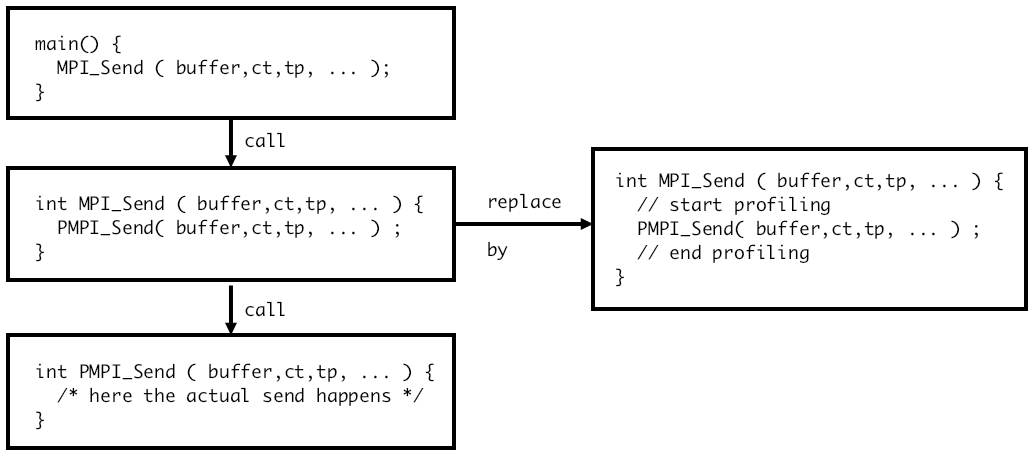
\includegraphics[scale=.5]{pmpi}
  \caption{Calling hierarchy of MPI and PMPI routines}
  \label{fig:pmpi-call}
\end{figure}
See figure~\ref{fig:pmpi-call}.

By default, the MPI routines are defined
as
\emph{weak linker symbols}\index{linker!weak symbol}\index{weak symbol|see{linker, weak symbol}}
as a synonym of the PMPI ones. In the gcc case:
\begin{verbatim}
#pragma weak MPI_Send = PMPI_Send
\end{verbatim}
\begin{figure}[ht]
  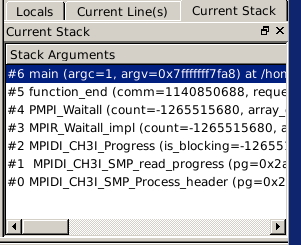
\includegraphics[scale=.7]{pmpi-trace}
  \caption{A stack trace, showing the \texttt{PMPI} calls.}
  \label{fig:pmpi-trace}
\end{figure}
As you can see in figure~\ref{fig:pmpi-trace}, normally only the \n{PMPI} routines
show up in the stack trace.

%% Does the standard mandate this?

\Level 1 {Tools interface}
\index{MPI!tools interface|(}

Recent versions of MPI have a standardized way of reading out
performance variables: the \emph{tools interface}
which improves on the old interface described in section~\ref{sec:profile}.

The realization of the tools interface is installation-dependent,
you first need to query how much of the tools interface is provided.

\cverbatimsnippet[code/mpi/c/mpit.c]{mpit_init_q}

\cverbatimsnippet[code/mpi/c/mpit.c]{mpit_list}

\index{MPI!tools interface|)}

\Level 1 {Programming for performance}

We outline some issues pertaining to performance.

\heading{Eager limit}

Short blocking messages are handled by a simpler mechanism than
longer. The limit on what is considered `short' is known as the
\indexterm{eager limit} (section~\ref{sec:eager-limit}), and you could
tune your code by increasing its value. However, note that a process
may likely have a buffer accomodating eager sends for every single
other process. This may eat into your available memory.

\heading{Blocking versus non-blocking}
%
The issue of \emph{blocking versus
  non-blocking}\index{communication!blocking!vs non-blocking}
communication is something of a red herring. While non-blocking
communication allows \indextermbus{latency}{hiding}, we can not
consider it an alternative to blocking sends, since replacing
non-blocking by blocking calls will usually give \indexterm{deadlock}.

Still, even if you use non-blocking communication for the mere
avoidance of deadlock or serialization
(section~\ref{sec:serialization}), bear in mind the possibility of
overlap of communication and computation. This also brings us to our
next point.

Looking at it the other way around, in a code with blocking sends you
may get better performance from non-blocking, even if that is not
structurally necessary.

\heading{Progress}

MPI is not magically active in the background, especially if the user
code is doing scalar work that does not involve MPI. As sketched in
section~\ref{sec:progress}, there are various ways of ensuring that
latency hiding actually happens.

\heading{Persistent sends}

If a communication between the same pair of processes, involving the
same buffer, happens regularly, it is possible to set up a
\indextermsub{persistent}{communication}. See section~\ref{sec:persistent}.

\heading{Buffering}

MPI uses internal buffers, and the copying from user data to these
buffers may affect performance. For instance, derived types
(section~\ref{sec:derived-types}) can typically not be streamed
straight through the network (this requires special hardware
support~\cite{LI:MpiDataUMR}) so they are first copied. Somewhat
surprisingly, we find that \indextermsub{buffered}{communication}
(section~\ref{sec:buffered}) does not help. Perhaps MPI implementors
have not optimized this mode since it is so rarely used.

This is issue is extensively investigated in~\cite{Eijkhout:MPItype-arxiv}.

\heading{Graph topology and neighborhood collectives}

Load balancing and communication minimization are important in
irregular applications. There are dedicated programs for this
(\indexterm{ParMetis}, \indexterm{Zoltan}), and libraries such as
\indexterm{PETSc} may offer convenient access to such capabilities.

In the declaration of a \indextermbus{graph}{topology}
  (section~\ref{sec:mpi-dist-graph}) MPI is allowed to
reorder processes, which could be used to support such activities.
It can also serve for better message sequencing when
\indextermsub{neighbourhood}{collectives} are used.

\heading{Network issues}

In the discussion so far we have assumed that the network is a perfect
conduit for data. However, there are issues of port design, in
particular caused by
\emph{oversubscription}\index{network!port!oversubscription} that
adversely affect performance. While in an ideal world it may be
possible to set up routine to avoid this, in the actual practice of a
supercomputer cluster, \indextermbus{network}{contention} or
\indextermbus{message}{collision} from
different user jobs is hard to avoid.

\heading{Offloading and onloading}
\index{offloading!vs onloading}\index{onloading|see{offloading, vs onloading}}

There are different philosophies of \indextermbus{network}{card}
\emph{design}: \indexterm{Mellanox}, being a network card manufacturer,
believes in off-loading network activity to the \ac{NIC}, while
\indexterm{Intel}, being a processor manufacturer, believes in
`on-loading' activity to the process. There are argument either way.

Either way, investigate the capabilities of your network.

\Level 1 {MPIR}

\indextermdef{MPIR} is the informally specified debugging interface
for processes acquisition and message queue extraction.

\Level 0 {Determinism}
\label{sec:mpi-semantics}
\index{MPI!semantics|(}

MPI processes are only synchronized to a certain extent, so you may
wonder what guarantees there are that running a code twice will give
the same result.  You need to consider two cases: first of all, if the
two runs are on different numbers of processors there are already
numerical problems; see~\HPSCref{sec:roundoff-parallel}.

Let us then limit ourselves to two runs on the same set of processors. 
In that case, MPI is deterministic as long as you do not use 
wildcards such as \indexmpishow{MPI_ANY_SOURCE}. Formally, 
MPI messages are `non-overtaking': two messages between the same
sender-receiver pair will arrive in sequence.
Actually, they may not arrive in sequence: they are \emph{matched}\index{matching}
in sequence in the user program. If the second message is much smaller than the first,
it may actually arrive earlier in the lower transport layer.

\index{MPI!semantics|)}

\Level 0 {Subtleties with processor synchronization}
\label{sec:handshake}

Blocking communication involves a complicated dialog between the two
processors involved. Processor one says `I~have this much data to
send; do you have space for that?', to which processor two replies
`yes, I~do; go ahead and send', upon which processor one does the
actual send. This back-and-forth (technically known as
a \indexterm{handshake}) takes a certain amount of communication
overhead. For this reason, network hardware will sometimes forgo the
handshake for small messages, and just send them regardless, knowing
that the other process has a small buffer for such occasions.

%This behaviour is not dictated by the standard: it is up to the implementation
%to make this optimization for small messages.

One strange side-effect of this strategy is that a code that
should \indexterm{deadlock} according to the MPI specification does
not do so. In effect, you may be shielded from you own programming
mistake! Of course, if you then run a larger problem, and the small
message becomes larger than the threshold, the deadlock will suddenly
occur. So you find yourself in the situation that a bug only manifests
itself on large problems, which are usually harder to debug.
In this case,
replacing every \indexmpishow{MPI_Send} with a \indexmpishow{MPI_Ssend}
will force the handshake, even for small messages.

Conversely, you may sometimes wish to avoid the handshake on large
messages. MPI as a solution for this: the \indexmpishow{MPI_Rsend} (`ready
send') routine sends its data immediately, but it needs the receiver
to be ready for this. How can you guarantee that the receiving process
is ready? You could for instance do the following (this uses
non-blocking routines, which are explained below in
section~\ref{sec:nonblocking}):
\begin{lstlisting}
if ( receiving ) {
  MPI_Irecv()   // post non-blocking receive
  MPI_Barrier() // synchronize
else if ( sending ) {
  MPI_Barrier() // synchronize
  MPI_Rsend()   // send data fast
\end{lstlisting}
When the barrier is reached, the receive has been posted, so it is safe 
to do a ready send. However, global barriers are not a good idea.
Instead you would just synchronize the two processes involved.
\begin{exercise}
  Give pseudo-code for a scheme where you synchronize the two
  processes through the exchange of a blocking zero-size message.
\end{exercise}

\Level 0 {Shell interaction}

MPI programs are not run directly from the shell, but are started
through an \indextermsub{ssh}{tunnel}. We briefly discuss
ramifications of this.

\Level 1 {Standard input}
\label{sec:mpi-stdin}

Letting MPI processes interact with the environment is not entirely
straightforward.
For instance,
\index{redirection|see{shell, input redirection}}%
\indextermsub{shell}{input redirection}
as in
\begin{verbatim}
mpirun -np 2 mpiprogram < someinput
\end{verbatim}
may not work.

Instead, use a script \n{programscript} that has one parameter:
\begin{verbatim}
#!/bin/bash
mpirunprogram < $1
\end{verbatim}
and run this in parallel:
\begin{verbatim}
mpirun -np 2 programscript someinput
\end{verbatim}

\Level 1 {Standard out and error}

The \indexterm{stdout} and \indexterm{stderr} streams of an MPI
process are returned through the ssh tunnel. Thus they can be caught
as the \indexterm{stdout/err of}{mpirun}.

\cverbatimsnippet[examples/mpi/c/outerr.c]{mpiouterr}

\Level 1 {Process status}

The return code of \indexmpishow{MPI_Abort} is returned as the
\indexterm{processes status of}{mpirun}.
Running
\cverbatimsnippet[examples/mpi/c/abort.c]{mpiabort37}
as
\begin{verbatim}
mpirun -np 4 ./abort ; \
echo "Return code from ${MPIRUN} is <<$$?>>"
\end{verbatim}
gives
\begin{verbatim}
TACC:  Starting up job 3760534
TACC:  Starting parallel tasks...
application called MPI_Abort(MPI_COMM_WORLD, 37) - process 3
TACC:  MPI job exited with code: 37
TACC:  Shutdown complete. Exiting.
Return code from ibrun is <<37>>
\end{verbatim}

\Level 1 {Multiple program start}
\label{sec:mpmd-start}

The sort of script of section~\ref{sec:mpi-stdin}
can also be used to implement \indexac{MPMD} runs:
we let the script start one of a number of programs. For this, we use
the fact that the MPI rank is known in the environment as
\indextermtt{PMI_RANK}. Use a script \n{mpmdscript}:
\begin{verbatim}
#!/bin/bash
if [ ${PMI_RANK} -eq 0 ] ; then
  ./programmaster
else
  ./programworker
fi
\end{verbatim}
which is then run in parallel:
\begin{verbatim}
mpirun -np 25 mpmdscript
\end{verbatim}

\Level 0 {The origin of one-sided communication in ShMem}

The \indextermbus{Cray}{T3E} had a library called \indexterm{shmem}
which offered a type of shared memory. Rather than having a true
global address space it worked by supporting variables that were
guaranteed to be identical between processors, and indeed, were
guaranteed to occupy the same location in memory. Variables could be
declared to be shared a `symmetric' pragma or directive; their values
could be retrieved or set by \n{shmem_get} and \n{shmem_put} calls.

\Level 0 {Leftover topics}

\Level 1 {MPI constants}
\index{MPI!constants|(}

MPI has a number of built-in \emph{constants}. These do not all behave
the same.
\begin{itemize}
\item Some are \emph{compile-time}\index{MPI!constants!compile-time}
  constants. Examples are \indexmpishow{MPI_VERSION} and
  \indexmpishow{MPI_MAX_PROCESSOR_NAME}. Thus, they can be used in
  array size declarations, even before \indexmpishow{MPI_Init}.
\item Some \emph{link-time}\index{MPI!constants!link-time}
  constants get their value by MPI initialization, such as
  \indexmpishow{MPI_COMM_WORLD}. Such symbols, which include all
  predefined handles, can be used in initialization expressions.
\item Some link-time symbols can not be used in initialization
  expressions, such as \indexmpishow{MPI_BOTTOM} and \indexmpishow{MPI_STATUS_IGNORE}.
\end{itemize}

For symbols, the binary realization is not defined. For instance,
\indexmpishow{MPI_COMM_WORLD} is of type \indexmpishow{MPI_Comm}, but
the implementation of that type is not specified.

See Annex~A of the \mpistandard{3.1} standard for full lists.

The following are the compile-time constants:
\begin{itemize}
\item \indexmpishow{MPI_MAX_PROCESSOR_NAME}
\item \indexmpishow{MPI_MAX_LIBRARY_VERSION_STRING}
\item \indexmpishow{MPI_MAX_ERROR_STRING}
\item \indexmpishow{MPI_MAX_DATAREP_STRING}
\item \indexmpishow{MPI_MAX_INFO_KEY}
\item \indexmpishow{MPI_MAX_INFO_VAL}
\item \indexmpishow{MPI_MAX_OBJECT_NAME}
\item \indexmpishow{MPI_MAX_PORT_NAME}
\item \indexmpishow{MPI_VERSION}
\item \indexmpishow{MPI_SUBVERSION}
\item \indexmpishow{MPI_STATUS_SIZE} (Fortran only)
\item \indexmpishow{MPI_ADDRESS_KIND} (Fortran only)
\item \indexmpishow{MPI_COUNT_KIND} (Fortran only)
\item \indexmpishow{MPI_INTEGER_KIND} (Fortran only)
\item \indexmpishow{MPI_OFFSET_KIND} (Fortran only)
\item \indexmpishow{MPI_SUBARRAYS_SUPPORTED} (Fortran only)
\item \indexmpishow{MPI_ASYNC_PROTECTS_NONBLOCKING}  (Fortran only)
\end{itemize}

The following are the link-time constants:
\begin{itemize}
\item \indexmpishow{MPI_BOTTOM}
\item \indexmpishow{MPI_STATUS_IGNORE}
\item \indexmpishow{MPI_STATUSES_IGNORE}
\item \indexmpishow{MPI_ERRCODES_IGNORE}
\item \indexmpishow{MPI_IN_PLACE}
\item \indexmpishow{MPI_ARGV_NULL}
\item \indexmpishow{MPI_ARGVS_NULL}
\item \indexmpishow{MPI_UNWEIGHTED}
\item \indexmpishow{MPI_WEIGHTS_EMPTY}
\end{itemize}

Assorted constants:
%% C type: const int (or unnamed enum)
%% Fortran type: INTEGER
\begin{itemize}
\item \indexmpishow{MPI_PROC_NULL}
\item \indexmpishow{MPI_ANY_SOURCE}
\item \indexmpishow{MPI_ANY_TAG}
\item \indexmpishow{MPI_UNDEFINED}
\item \indexmpishow{MPI_BSEND_OVERHEAD}
\item \indexmpishow{MPI_KEYVAL_INVALID                }
\item \indexmpishow{MPI_LOCK_EXCLUSIVE}
\item \indexmpishow{MPI_LOCK_SHARED}
\item \indexmpishow{MPI_ROOT}
\end{itemize}

(This section was inspired by
\url{http://blogs.cisco.com/performance/mpi-outside-of-c-and-fortran}.)

\index{MPI!constants|)}

\Level 1 {32-bit size issues}

The \n{size} parameter in MPI routines is defined as an \n{int},
meaning that it is limited to 32-bit quantities.  There are ways
around this, such as sending a number of
\indexmpishow{MPI_Type_contiguous} blocks that add up to more than~$2^{31}$.

\Level 1 {Python issues}
\label{sec:python-stuff}
\index{MPI!Python issues|(}

\Level 2 {Byte calculations}

The \indexmpishow{MPI_Win_create} routine needs a displacement in
bytes. Here is a good way for finding the size of \indexterm{numpy} datatypes:
\lstset{language=Python} %pyskip
\begin{lstlisting}
numpy.dtype('i').itemsize
\end{lstlisting}

\Level 2 {Arrays of objects}

Objects of type \lstinline{MPI.Status} or \lstinline{MPI.Request} often need to be created
in an array, for instance when looping through a number of \n{Isend} calls.
In that case the following idiom may come in handy:

\lstset{language=Python} %pyskip
\begin{lstlisting}
requests = [ None ] * nprocs
for p in range(nprocs):
  requests[p] = comm.Irecv( ... )
\end{lstlisting}
\lstset{language=C} %pyskip

\index{MPI!Python issues|)}

\Level 1 {Cancelling messages}

In section~\ref{sec:mpi-source} we showed a master-worker example where the 
master accepts in arbitrary order the messages from the workers.
Here we will show a slightly
more complicated example, where only the result of the first task to
complete is needed. Thus, we issue an \indexmpishow{MPI_Recv}
with \indexmpishow{MPI_ANY_SOURCE} as source.  When a result comes, we
broadcast its source to all processes.  All the other workers then use
this information to cancel their message with
an \indexmpishow{MPI_Cancel} operation.
%
\cverbatimsnippet[examples/mpi/c/cancel.c]{cancel}

After the cancelling operation it is still necessary to call
\indexmpishow{MPI_Request_free}, \indexmpishow{MPI_Wait}, or
\indexmpishow{MPI_Test} in order to free the request object.

The \indexmpishow{MPI_Cancel} operation is local, so it can not be
used for \emph{non-blocking
  collectives}\index{collectives!non-blocking!cancelling} or one-sided transfers.

\begin{remark}
  As of \mpistandard{3.2}, cancelling a send is deprecated.
\end{remark}

\Level 1 {Constants}

MPI constants such as \indexmpishow{MPI_COMM_WORLD} or \indexmpishow{MPI_INT} are not
necessarily statitally defined, such as by a \n{#define} statement:
the best you can say is that they have a value after
\indexmpishow{MPI_Init} or \indexmpishow{MPI_Init_thread}.
That means you can not transfer a compiled MPI file between
platforms, or even between compilers on one platform.
However, a working MPI source on one MPI implementation
will also work on another.

\Level 0 {Literature}

Online resources:
\begin{itemize}
\item MPI 1 Complete reference:\\ \url{http://www.netlib.org/utk/papers/mpi-book/mpi-book.html}
\item Official MPI documents:\\ \url{http://www.mpi-forum.org/docs/}
\item List of all MPI routines:\\ \url{http://www.mcs.anl.gov/research/projects/mpi/www/www3/}
\end{itemize}

Tutorial books on MPI:
\begin{itemize}
\item Using MPI~\cite{Gropp:UsingMPI1} by some of the original authors.
\end{itemize}

\endinput

Examples: 
compute pi
mandelbrot set
